

\chapter{Results}
% o Present all results here
% o No discussion, no interpretation, no evaluation etc.
% o Figures / Tables
%  Use wisely
%  Consult your supervisor about what to present
%  put very large and detailed tables rather in the appendix
%  put source code in appendix
% o Do not write down all data from table in text, but put them in relation to each other
% o Help reader to understand tables & graphs and highlight important and/or interesting data
% o Present an assessment of uncertainties

On the second day of working with the filled rods the one containing liquid \textbf{\#6} broke (leakage).
It happened when delicately knocking it against on the table while standing upright.
This was intended to mobilise bubbles that sticked to the wall and make them travel vertically to on end of the rod. (see table \ref{tab:bubbles})
The plastic stopper on the lower end came loose.
The rod containing filling \textbf{\#6} was not replaced.
Consequently, all CT/MRI images used to asses signal intensities of the tested solutions show only 16 rods.

\section{Obtained MRI and CT scans}
Figure \ref{fig:coronal} shows a coronal view of the 16 rods filled with the tested liquids and a reference rod on either side.
In Figure \ref{fig:coronal_MR} a trapped air bubble is clearly visible at the lower half of rod \#5.
Figure \ref{fig:axial} shows an axial view of the tested rods and some surrounding rods.
In figure \ref{fig:axial_MR} a water filled plastic bottle placed in the middle of the phantom is also visible.
This was necessary, because the MRI scanner needs sufficient signal to start imaging.
Without the bottle, the limited number of rods used for this scan would not have created enough signal.
During a future distortion assessment where all available rods (over 300) would be used, they are supposed to result in the required signal strength on their own.
 
\begin{figure}[!tbp]
  \begin{subfigure}[b]{\textwidth}
    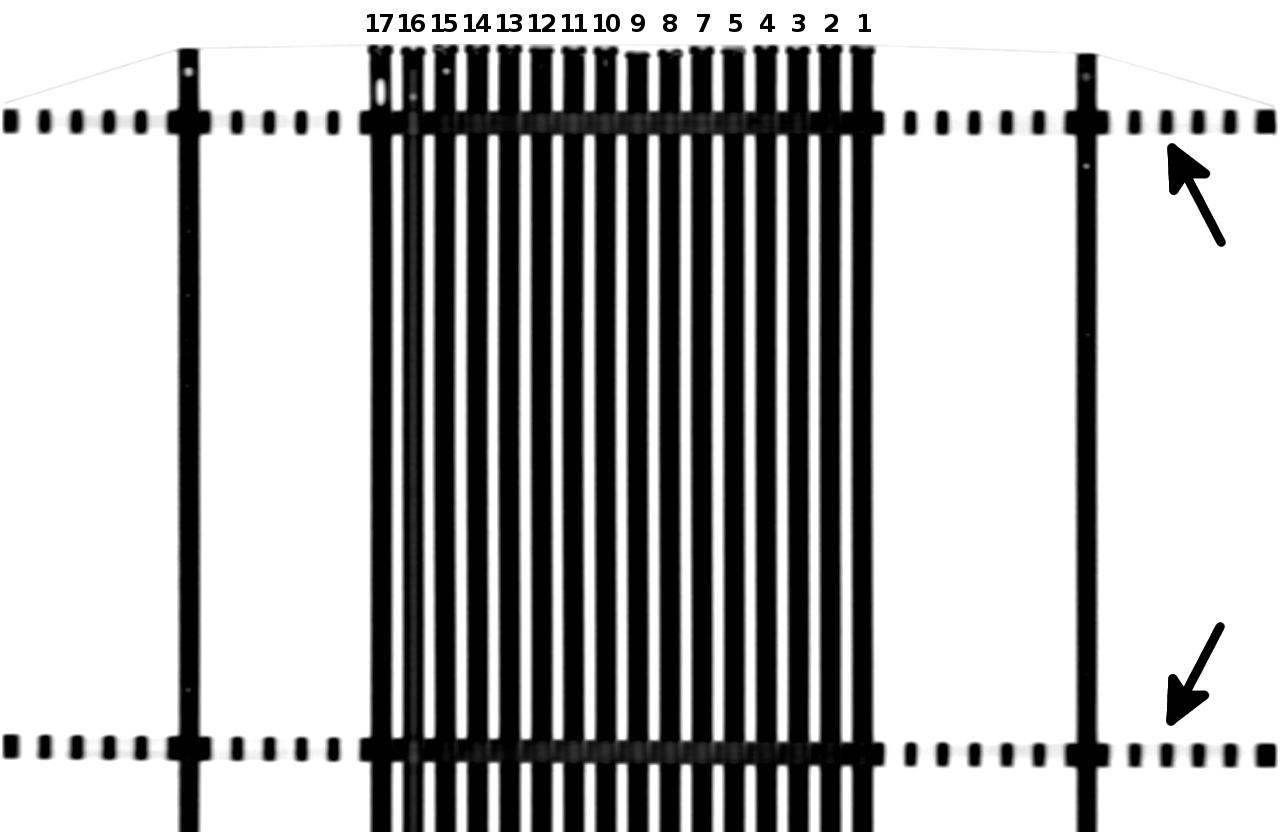
\includegraphics[width=\textwidth]{slicer3D/full_phantom/coronal_CT_cropped-arrow.png}
    \caption{CT: The periodic black lines in upper and lower part of image (indicated with arrows) depict the plastic panes and their holes from above; The faint line across upper end of rods shows adhesive tape used to hold the rods in place; In rod \#17 an air bubble is clearly visible close to the upper end.}
    \label{fig:coronal_CT}
  \end{subfigure}
  \begin{subfigure}[b]{1\textwidth}
    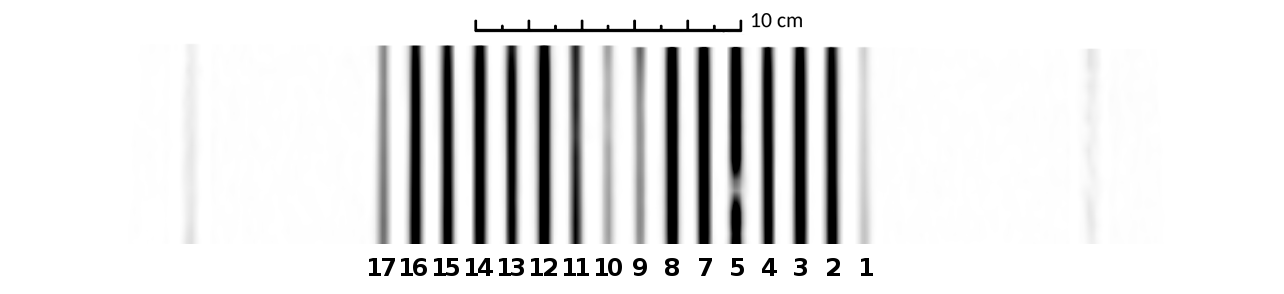
\includegraphics[width=1\textwidth]{slicer3D/full_phantom/coronal_MR_cropped.png}
    \caption{MR: The rods appear to be thinner than in the CT scan, because only the liquid filling is visible. The tested liquids result in different signal intensity (brightness); all plastic parts (rods and panes) are not visible; there is a trapped air bubble visible in rod \#5.}
    \label{fig:coronal_MR}
  \end{subfigure}
  \caption{Coronal CT/MRI (inverted colours; same scale; cropped images) images of 16 rods (tested liquids, numbering starting from the right, \#6 excluded) + 2 reference rods (filled with water) on the sides.}
  \label{fig:coronal}
\end{figure}

\begin{figure}[!tbp]
  \begin{subfigure}[b]{\textwidth}
    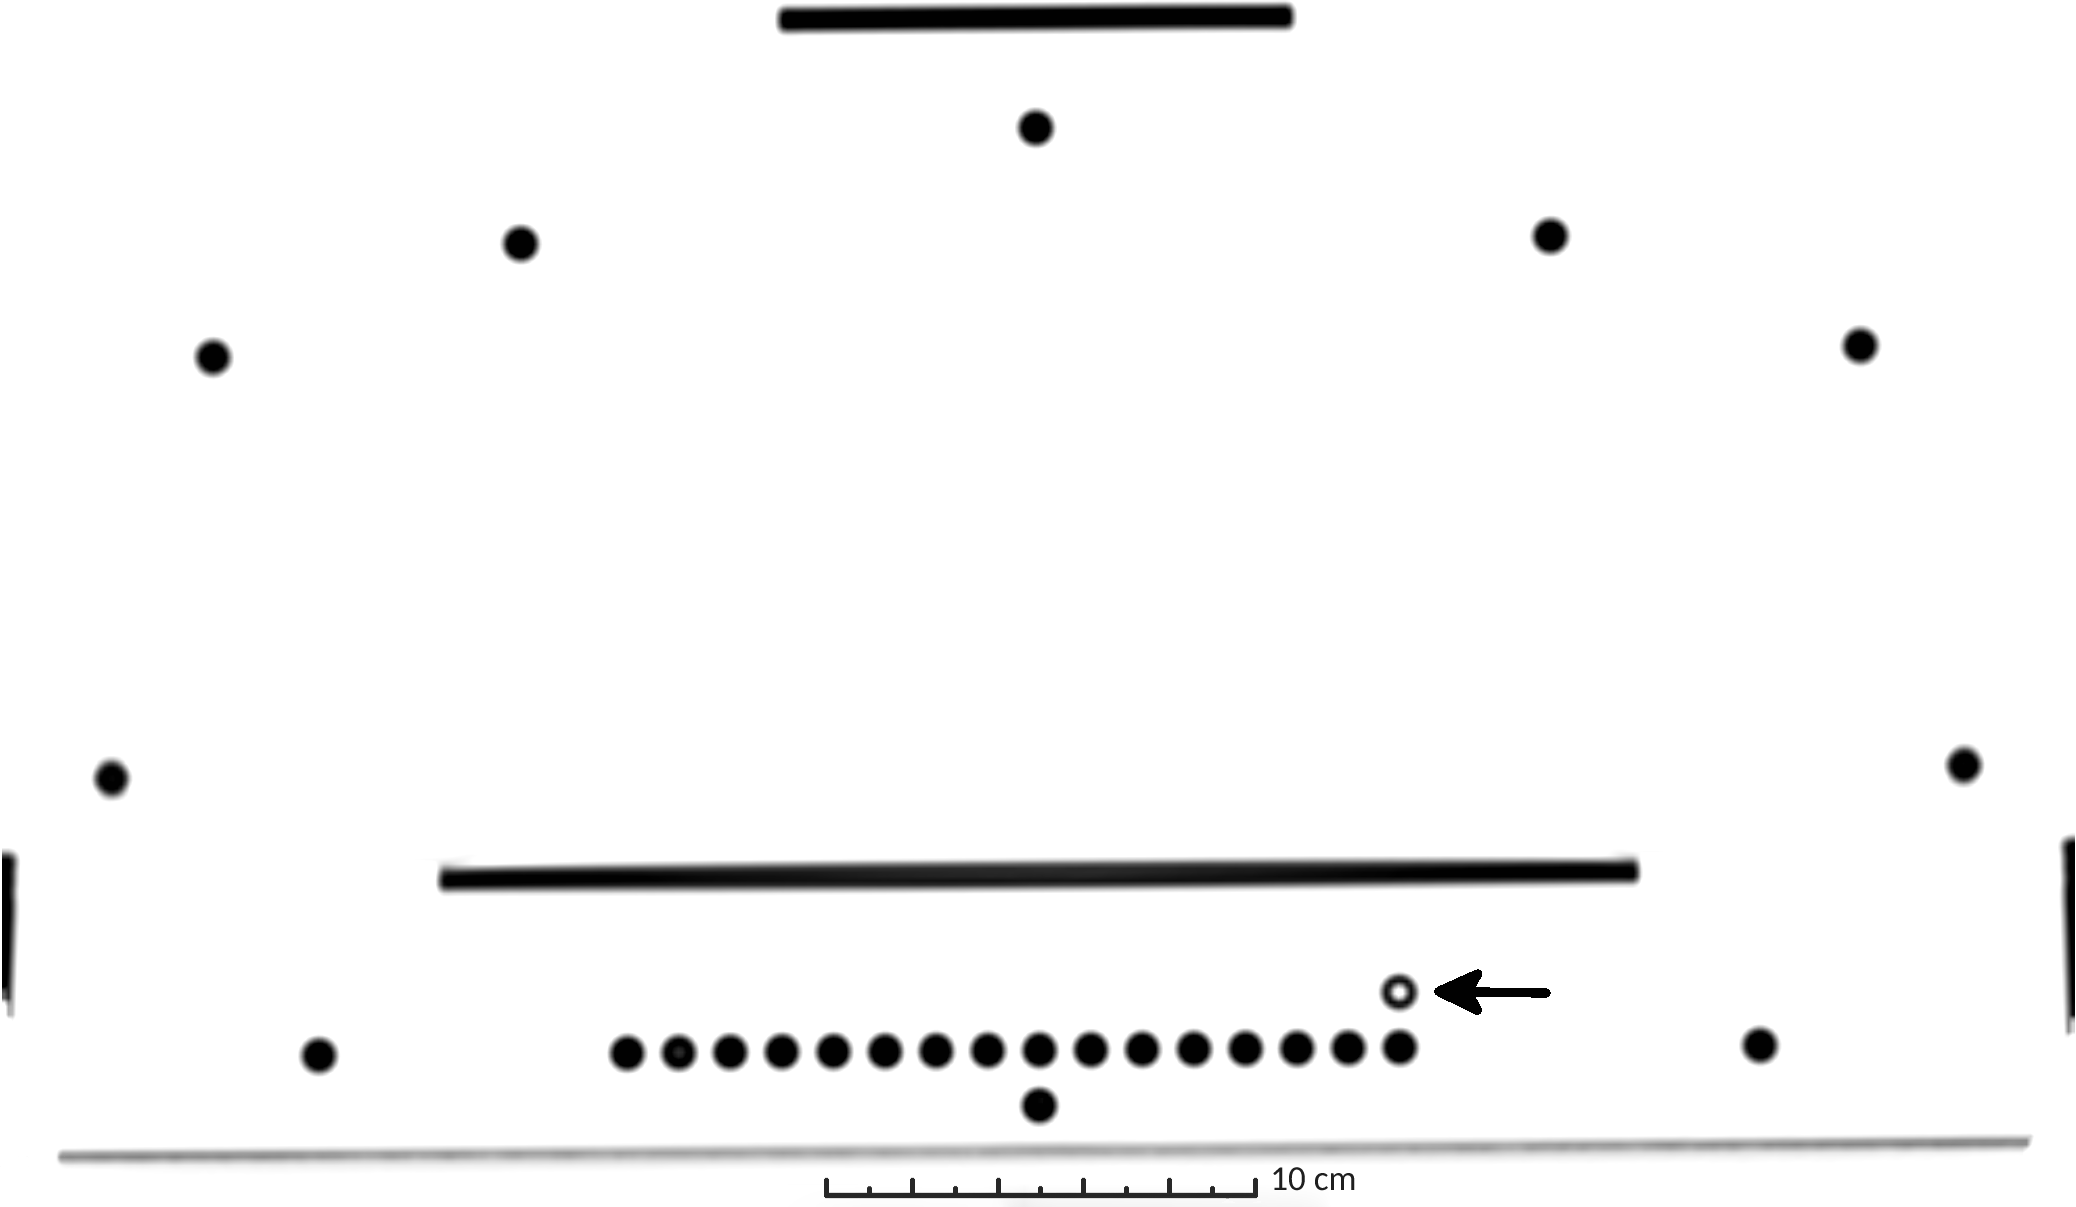
\includegraphics[width=\textwidth]{slicer3D/full_phantom/axial_CT_rods-arrow.png}
    \caption{CT: The black bars visible just above the 16 tested rods, at the very top, and to the sides show plastic parts of the phantom holding it together. The faint grey line running below the tested rods represents the table on which the phantom was positioned during imaging.}
    \label{fig:axial_CT_rods}
  \end{subfigure}
  \begin{subfigure}[b]{\textwidth}
    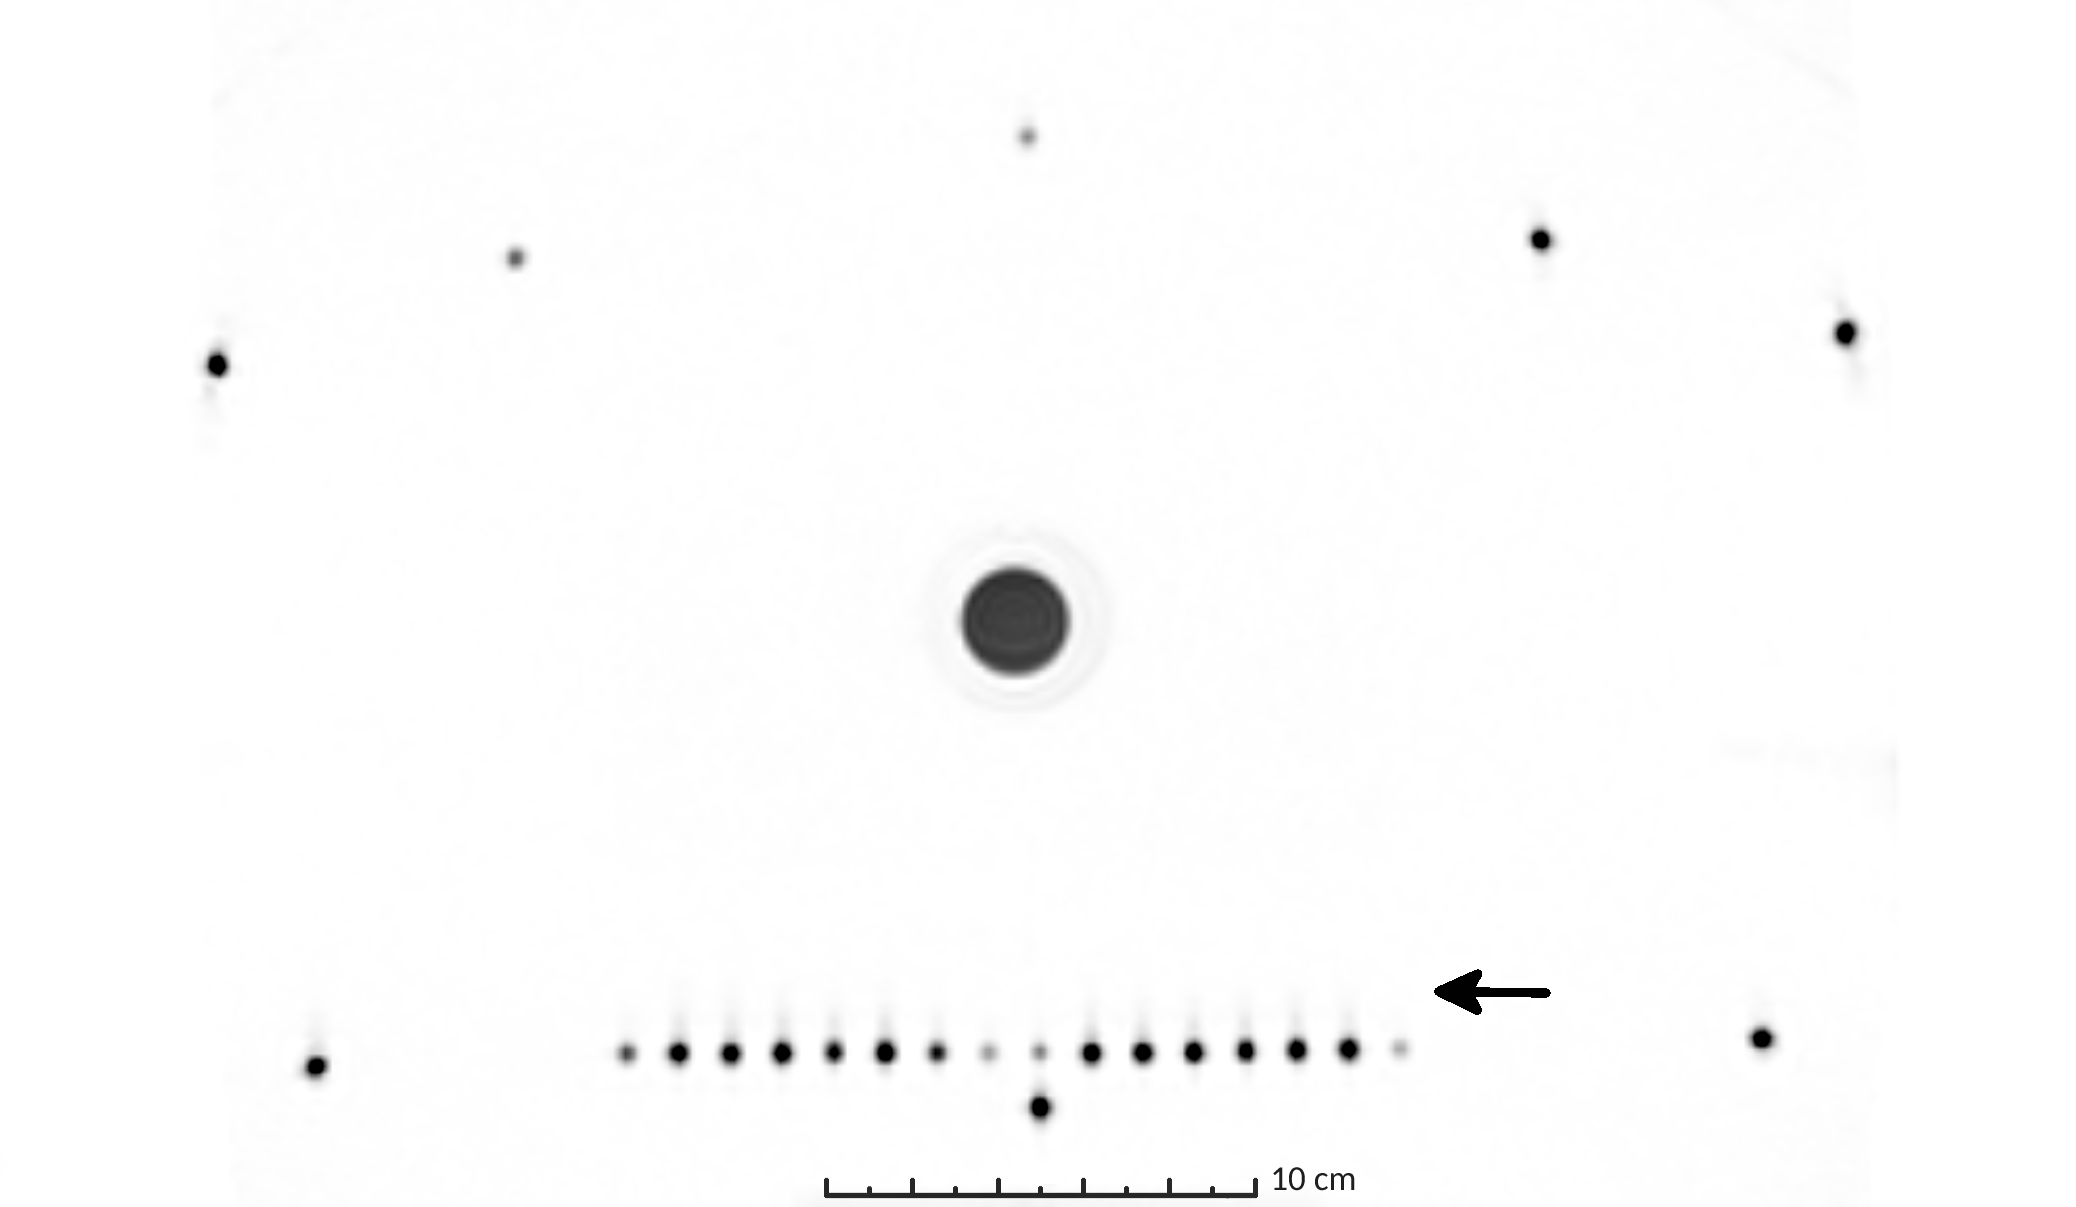
\includegraphics[width=\textwidth]{slicer3D/full_phantom/axial_MR-arrow.png}
    \caption{MRI: The black circle in the centre depicts a water bottle which was placed in the middle of the phantom (necessary for MRI scanner to start imaging).}
    \label{fig:axial_MR}
  \end{subfigure}
  \caption{axial CT/MRI (inverted colours, same scale) images of the 16 rods filled with tested liquids (numbering starting from the right, \#6 excluded); surrounded by reference rods (filled with water) and one empty rod (marked with arrow) which is not visible on the MRI scan}
  \label{fig:axial}
\end{figure}


\section{Tested solutions}

\subsection{Visibility on CT/MRI scans}

It should be noticed that in the CT image there is little difference in brightness between the tested liquids.
The plastic rods themselves result in brighter pixels than any of the tested solutions.

On MRI scans most liquids had a mean and a max brightness value above $1000$ (see table \ref{tab:visibility}).\\
Only \textbf{\#1}, \textbf{\#9}, \textbf{\#10}, \& \textbf{\#17} resulted in significantly less signal (below < $1000$).


\begin{table}[!htb]
\centering
\begin{tabular}{@{}l|lllll@{}}
\toprule
No. & Min  & Max  & Mean   & Median & $\sigma$ \\ \midrule
1   & 182  & 371  & 288    & 269    & 69,8     \\
2   & 1044 & 1921 & 1443,8 & 1405   & 312,9    \\
3   & 941  & 2075 & 1451,2 & 1394,5 & 413,2    \\
4   & 1176 & 1709 & 1440   & 1437,5 & 232,5    \\
5   & 1125 & 2111 & 1583,8 & 1549,5 & 355      \\
7   & 971  & 2241 & 1466,8 & 1316   & 471,2    \\
8   & 1459 & 1947 & 1704   & 1705   & 180,5    \\
9   & 385  & 584  & 486,8  & 489    & 93       \\
10  & 247  & 502  & 343,6  & 266    & 111      \\
11  & 830  & 1268 & 1036,2 & 1023,5 & 163,2    \\
12  & 1158 & 2211 & 1648,8 & 1613   & 394,2    \\
13  & 836  & 1657 & 1146,8 & 1047   & 321,2    \\
14  & 800  & 2062 & 1383   & 1335   & 473,1    \\
15  & 1156 & 1829 & 1476,2 & 1460   & 272,7    \\
16  & 1102 & 1967 & 1509   & 1483,5 & 325,8    \\
17  & 356  & 938  & 629,6  & 602    & 223,6    \\ \bottomrule
\end{tabular}
\caption{liquid visibility on MRI scan}
\label{tab:visibility}
\end{table}

\clearpage

\subsection{Mechanical properties of solutions}
\label{sec:sol-mech}

The liquids were filled in a rod each and observed for several months.
Number \textbf{\#14} could be injected without problems, the solution remained fluid even after reaching room temperature.
Number \textbf{\#15} on the other hand changed to a gel like consistence and clogged the injection tube at the quickly after the rod was filled.
The tube could not be used again.

Each rod was free of bubbles directly after sealing.
All rods containing water based solutions contained some air after 2 months and the amount of liquid continued to decrease further (see table \ref{tab:bubbles}).
In some of the tested rods the produced air bubbles would stick to the wall. Only after gently hitting the rod they would start moving.
Knowing the inner diameter $d$ of the rods and measuring the length $l$ of trapped air bubbles, we can approximate the volume of contained gas:

\begin{align}
 V = \frac{d^2}{4}\cdot \pi \cdot l
\end{align}

\begin{table}[]
\centering
\begin{tabular}{l|lc|lc|lc}
    & \multicolumn{2}{c}{\textit{after 1 day}} 	& \multicolumn{2}{c}{\textit{after 2 days}}	& \multicolumn{2}{c}{\textit{after 1 week}}	\\ 
No. & bubbles	& hit req.	& bubbles 	& hit req.	& bubbles 	& hit req.	\\
\toprule
\#1   & yes	& no		& no		&		& no		&		\\
\#2   & yes	& yes		& no		&		& no		&		\\
\#3   & yes	& yes		& no		&		& no		&		\\
\#4   & yes	& yes		& no		&		& no		&		\\
\#5   & yes	& no		& yes		& no		& no		&		\\
\#6   & yes	& no		& \multicolumn{4}{l}{-----------------\textit{ rod was leaking }------------------}	\\
\#7   & yes	& no		& yes		& no		& yes		& no		\\
\#8   & no	&		& no		&		& no		&		\\
\#9   & no	&		& no		&		& no		&		\\
\#10  & no$^1$	&		& yes		& yes		& yes		& yes		\\
\#11  & no	&		& yes,		& \textit{sticked to wall} &	 yes	& yes\\
\#12  & yes	& yes		& yes,		& \textit{sticked to wall} &	 yes	& yes\\
\#13  & yes	& yes		& yes,		& \textit{sticked to wall} &	 yes	& yes\\
\#14  & no	&   		& yes		& no		& yes		& yes		\\
\#15  & no	&   		& no		&		& no		&		\\
\#16  & no	&   		& no		&		& no		&		\\
\#17  & no	&   		& no		&		& no		&		\\
\bottomrule
\end{tabular}
\begin{tabular}{l|lr}
\multicolumn{3}{c}{}								\\
& \multicolumn{2}{c}{\textit{after 2 months}}					\\ 
No. & length of trapped bubble $l$ [$mm$] 	& approx. volume $V$ [$mm^3$]	\\
\toprule
\#1   & 2					& 25.13				\\
\#2   & 1.8					& 22.62				\\
\#3   & 1+1 (air blockage, at lower end)	& 25.13				\\
\#4   & 4					& 50.27				\\
\#5   & 1.5 (many small bubbles)		& 18.85				\\
\#6   & \multicolumn{2}{c}{-----------------------------\textit{ rod was leaking }------------------------------}\\
\#7   & 2 (many small bubbles)			& 25.13				\\
\#8   & 2.3					& 28.90				\\
\#9   & 3					& 37.70				\\
\#10  & 2.4					& 30.16				\\
\#11  & 2					& 25.13				\\
\#12  & 2					& 25.13				\\
\#13  & 2.3					& 28.90				\\
\#14  & 1.5+0.5 (big immobile bubble, at center)	& 25.13				\\
\#15  & 3.4 (agar gel dried)			& 42.73				\\
\#16  & 0					& 0.00				\\
\#17  & 0.5					& 6.28				\\
\bottomrule
\end{tabular}
\caption{Observations regarding the mechanical properties of the tested solutions.}
\label{tab:bubbles}
\end{table}


While adding generic washing soap (\textbf{\#5}, \textbf{\#6}, and \textbf{\#7}) did not hinder air bubbles from forming, it significantly improved their mobility.
Not only did they move quickly when the rod was tilted, large quantities of air also did not block the entire diameter of the rod.
Instead they formed large but cohesive bubbles that could be moved to one end of the rod easily and at no point sticked to the plastic wall.

The ascorbic acid present in \textbf{\#8} (concentration of $0.36 \; g/L$ corresponds to approx. $0.00204 \; mol/L$), \textbf{\#9} ($3.6 g/L$), and \textbf{\#10} ($36 g/L$) seemed to have held back the formation of air bubbles for up to one week.
After two months of observation, however, the rods also contained some air.
It should be noted that all three liquids turned brown, the colour being more saturated for higher concentrations of ascorbic acid.

The rods filled with Primovist (\textbf{\#11} to \textbf{\#13}) were filled with some air bubbles after at least two days.
Moreover, the bubbles sticked to the walls of the rod and only shaking it violently made them move to one side of the rod.

It took more than a week until the rod containing the low concentration of agar (\textbf{\#14}) contained an air bubble.
The viscous consistency made it impossible to coerce it to either end of the rod.
Liquid \textbf{\#15} on the other hand did not form bubbles at the middle of the rod, but seemed to have dried starting at the end with the plastic stopper.


\section{Distortion assessment}
All results were obtained by manually cropping the 3D image to depict only a single rod.
%As described later, resolution might influence the efficiency of the distortion assessment.#	
%Therefore all calculations were done with the original resolution and interpolated images that have a higher resolution.

\subsection{rod \#5}

The first scans were not only used to asses the brightness of the different solutions, but also to calculate occurring distortion.
As an example, the rod containing liquid \#5 was analysed.
Table \ref{tab:spit-out-5} shows the most interesting areas of the rod.


The obtained dice coefficient varies not only because of the circle's centre and the radius, it also depends on the images resolution.
Figure \ref{fig:CT_dc} and \ref{fig:MR_dc} show the DC (optimised) obtained using CT and MRI scans over resample rate.

 \begin{table}[p]
    \centering
    \rotatebox{90}{
      \begin{minipage}{\textheight}\footnotesize
        \centering
 \begin{tabular}{rr|lll|ll|llll}
 slice	& dist [$mm$]	& $warp_x$ [$mm$]	& $warp_y$ [$mm$]	& $warpMagnitude$ [$mm$]	& $DC_{CT}$	& $DC^*_{CT}$	& $DC_{MR}$	& $DC^*_{MR}$	& $DC_{MR(CT-COM)}$	& $DC^*_{MR(CT-COM)}$\\ \hline
 0      & -183			& -0.1032			& -1.1191			& 1.1239					& 0.9942	& 0.9942		& 0.7926	& 0.8213		& 0.5894			& 0.5908			\\
 1      & -182			& -0.1192			& -1.1175			& 1.1238					& 0.9932	& 0.9932		& 0.8031	& 0.8319		& 0.5953			& 0.5968			\\
 2      & -181			& -0.1265			& -1.1149			& 1.122 					& 0.9922	& 0.9922		& 0.8128	& 0.8418		& 0.6031			& 0.6049			\\
 :      &     			&        			&        			&       					&       	&       		&       	&       		&       			&       			\\
 \hline
 :      &     			&        			&        			&       					&       	&       		&       	&       		&       			&       			\\
 171    & -12 			& 0.0011 			& -0.6894			& 0.6894					& 0.9883	& 0.9883		& 0.9498	& 0.9475		& 0.7543			& 0.7548			\\
 172    & -11 			& 0.0075 			& -0.6827			& 0.6828					& 0.9847	& 0.9847		& 0.949 	& 0.9475		& 0.7541			& 0.7554			\\
 173    & -10 			& -1     			& -1     			& -1    					& -1    	& -1    		& 0.9498	& 0.9475		& -1    			& -1    			\\
 :      & :   			& :      			& :      			& :     					& :     	&       		&       	& :     		& :     			& :     			\\
 \hline &     			&        			&        			&       					&       	&       		&       	&       		&       			&       			\\
 :      & :   			& :      			& :      			& :     					& :     	&       		&       	& :     		& :     			& :     			\\
 193    & 10  			& -1     			& -1     			& -1    					& -1    	& -1    		& 0.9522	& 0.9539		& -1    			& -1    			\\
 194    & 11  			& 0.0368 			& -0.7094			& 0.7104					& 0.9834	& 0.9834		& 0.9542	& 0.9536		& 0.7611			& 0.7634			\\
 195    & 12  			& 0.0353 			& -0.7052			& 0.706 					& 0.9852	& 0.9852		& 0.9546	& 0.954 		& 0.7614			& 0.7637			\\
 :      &     			&        			&        			&       					&       	&       		&       	&       		&       			&       			\\
 \hline
 :      &     			&        			&        			&       					&       	&       		&       	&       		&       			&       			\\
 301    & 118 			& 0.3212 			& -0.8604			& 0.9184					& 0.9843	& 0.9843		& 0.3505	& 0.3681		& 0.3417			& 0.3496			\\
 302    & 119 			& 0.4215 			& -1.1644			& 1.2383					& 0.9859	& 0.9859		& 0.03  	& 0.0318		& 0.03  			& 0.0318			\\
 303    & 120 			& -1     			& -1     			& -1    					& 0.9864	& 0.9864		& -1    	& -1    		& 0     			& 0     			\\
 304    & 121 			& -1     			& -1     			& -1    					& 0.9877	& 0.9877		& -1    	& -1    		& 0     			& 0     			\\
 305    & 122 			& -1     			& -1     			& -1    					& 0.9897	& 0.9897		& -1    	& -1    		& 0     			& 0     			\\
 306    & 123 			& -1     			& -1     			& -1    					& 0.9891	& 0.9891		& -1    	& -1    		& 0     			& 0     			\\
 307    & 124 			& -1     			& -1     			& -1    					& 0.991 	& 0.991 		& -1    	& -1    		& 0     			& 0     			\\
 308    & 125 			& -1     			& -1     			& -1    					& 0.9873	& 0.9873		& -1    	& -1    		& 0     			& 0     			\\
 309    & 126 			& -1     			& -1     			& -1    					& 0.9918	& 0.9918		& -1    	& -1    		& 0     			& 0     			\\
 310    & 127 			& 0.3916 			& -2.0083			& 2.0461					& 0.9868	& 0.9868		& 0.0315	& 0.0334		& 0.0045			& 0     			\\
 311    & 128 			& 0.3627 			& -1.9906			& 2.0233					& 0.9933	& 0.9933		& 0.1149	& 0.1215		& 0.0546			& 0.044 			\\
 :      &     			&        			&        			&       					&       	&       		&       	&       		&       			&       			\\
 \hline
 :      &     			&        			&        			&       					&       	&       		&       	&       		&       			&       			\\
 393    & 210 			& 0.1105 			& -0.2561			& 0.2789					& 0.9862	& 0.9862		& 0.9132	& 0.9274		& 0.8751			& 0.8864			\\
 394    & 211 			& 0.117  			& -0.2628			& 0.2877					& 0.994 	& 0.994 		& 0.9132	& 0.9274		& 0.8768			& 0.889 			\\
 395    & 212 			& 0.1237 			& -0.2453			& 0.2747					& 0.9944	& 0.9944		& 0.9127	& 0.9278		& 0.8771			& 0.8894			 
 \end{tabular}
        \caption{rod \#5: script generated data}
        \label{tab:spit-out-5}
      \end{minipage}
    }
  \end{table}
 


\begin{figure}[!tbp]
  \begin{subfigure}[b]{0.32\textwidth}
    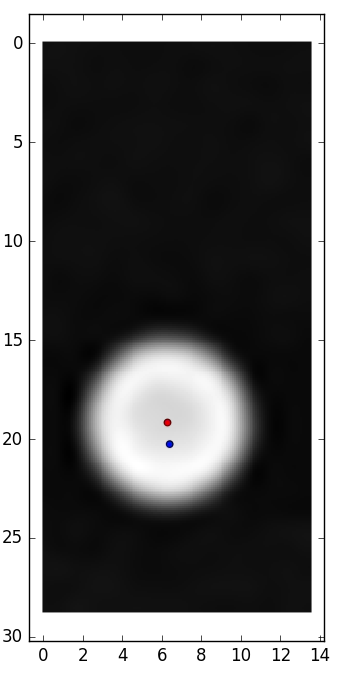
\includegraphics[scale=0.55]{python/ph2/centroid/CT_x100@0_centroids.png}
    \caption{CT @ 0}
    \label{fig:CT_x100_centroids@0}
  \end{subfigure}
  \begin{subfigure}[b]{0.32\textwidth}
    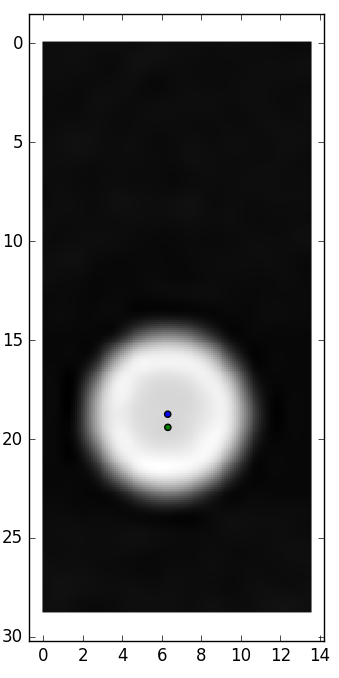
\includegraphics[scale=0.55]{python/ph2/centroid/CT_x100@150_centroids.png}
    \caption{CT @ 150}
    \label{fig:CT_x100_centroids@150}
  \end{subfigure}
  \begin{subfigure}[b]{0.32\textwidth}
    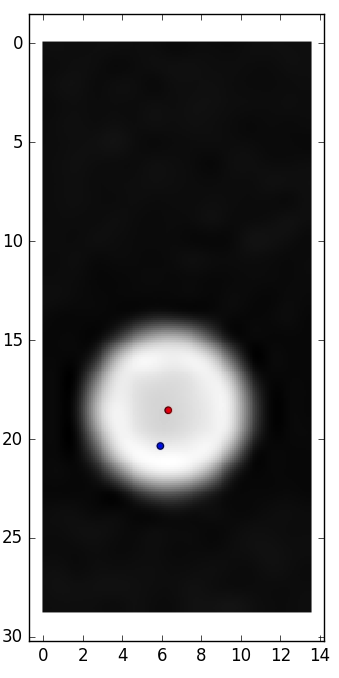
\includegraphics[scale=0.55]{python/ph2/centroid/CT_x100@304_centroids.png}
    \caption{CT @ 304}
    \label{fig:CT_x100_centroids@304}
  \end{subfigure}
  \begin{subfigure}[b]{0.32\textwidth}
    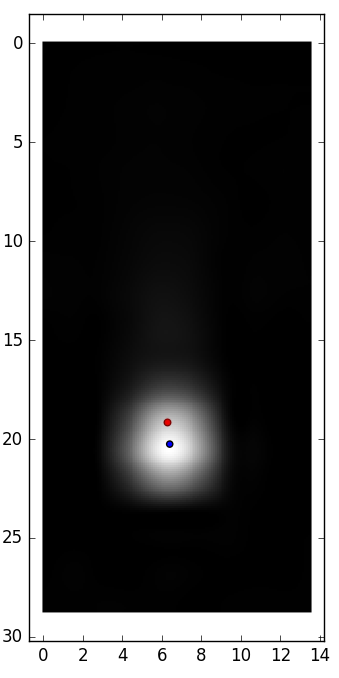
\includegraphics[scale=0.55]{python/ph2/centroid/MR_x100@0_centroids.png}
    \caption{MRI @ 0}
    \label{fig:MR_x100_centroids@0}
  \end{subfigure}
  \begin{subfigure}[b]{0.32\textwidth}
    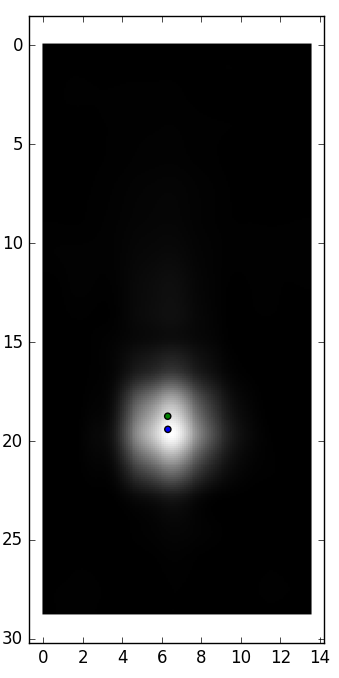
\includegraphics[scale=0.55]{python/ph2/centroid/MR_x100@150_centroids.png}
    \caption{MRI @ 150}
    \label{fig:MR_x100_centroids@150}
  \end{subfigure}
  \begin{subfigure}[b]{0.32\textwidth}
    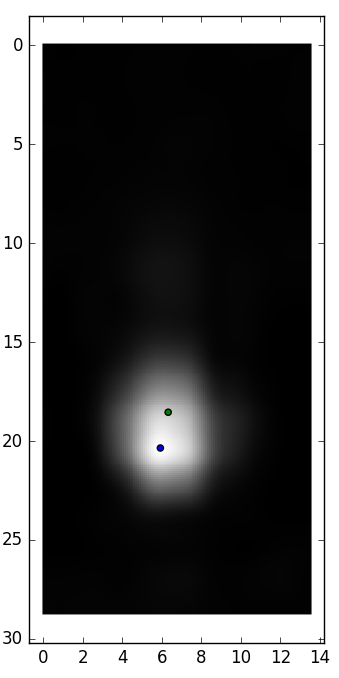
\includegraphics[scale=0.55]{python/ph2/centroid/MR_x100@304_centroids.png}
    \caption{MRI @ 304}
    \label{fig:MR_x100_centroids@304}
  \end{subfigure}
  \caption{MRI x100 scan of rod filled with \#5. The dark blue dot represents the MRI centroid, the bright red dot represents the CT centroid.
  			\\ Slice 150 is located approximately at the isocentre, 0 on the very end of the image, 304 on the other but also close to an air bubble.}
  \label{fig:MR_x100_centroids}
\end{figure}


\begin{figure}[!bp]
  \centering
  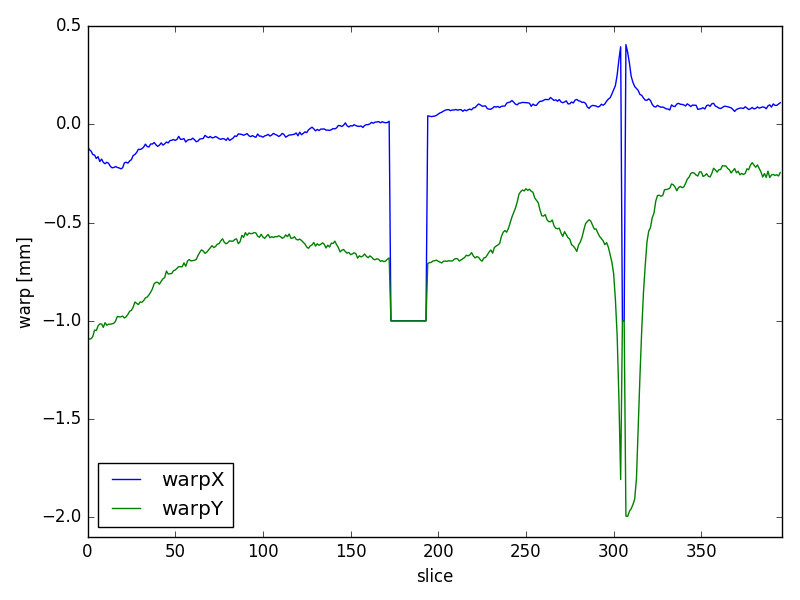
\includegraphics[scale=0.6]{python/ph2/warp/warpXY_x100--.png}
  \caption{warp XY [$mm$], CT-MRI x100}
  \label{fig:warpXY_x100}
\end{figure}

\begin{figure}[!tp]
    \centering
    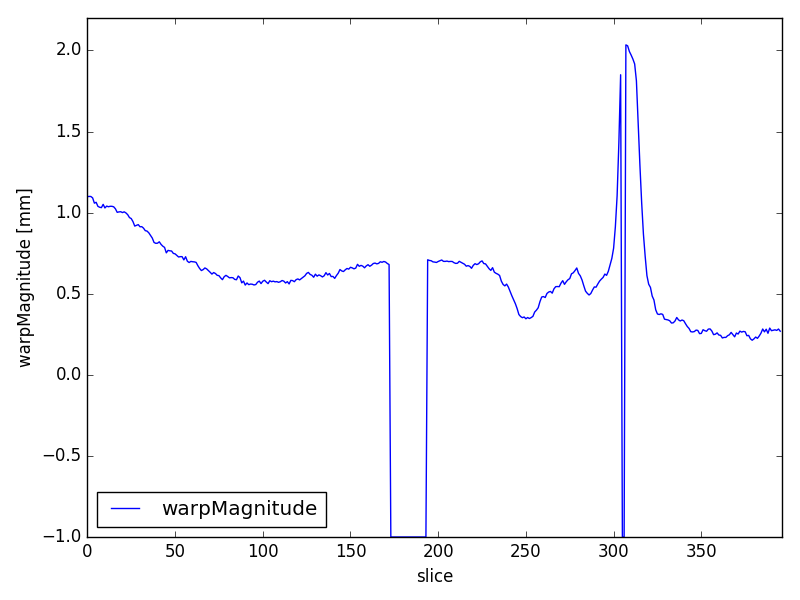
\includegraphics[scale=0.6]{python/ph2/warp/warpMagnitude_x100--.png}
    \caption{warp Magnitude [$mm$], CT-MRI x100}
    \label{fig:warpMagnitude_x100}
\end{figure}
\begin{figure}[!bp]
    \centering
    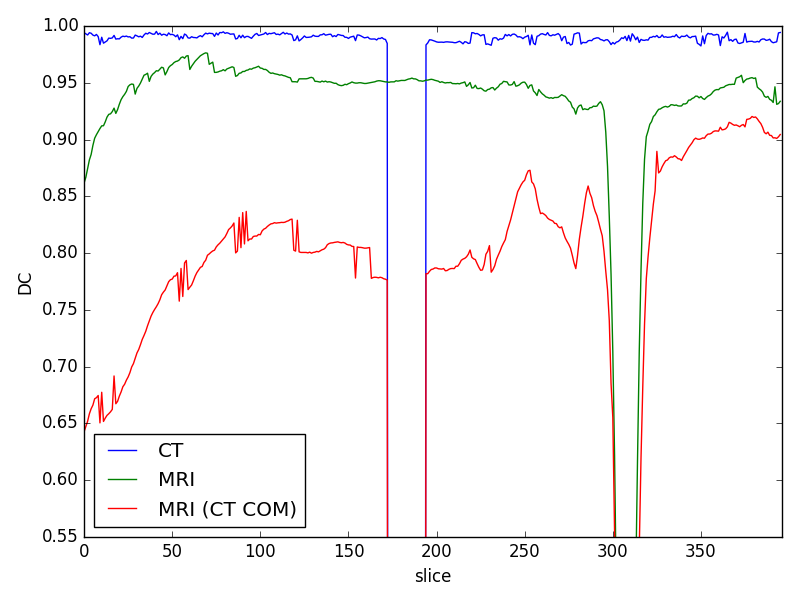
\includegraphics[scale=0.6]{python/ph2/dice/CT_MR_x100_DC.png}
    \caption{DC (optimised) for CT \& MRI \& MRI (using CT COM)}
    \label{fig:CT_MR_x100_DC}
\end{figure}

\begin{figure}[!bp]
  \centering
  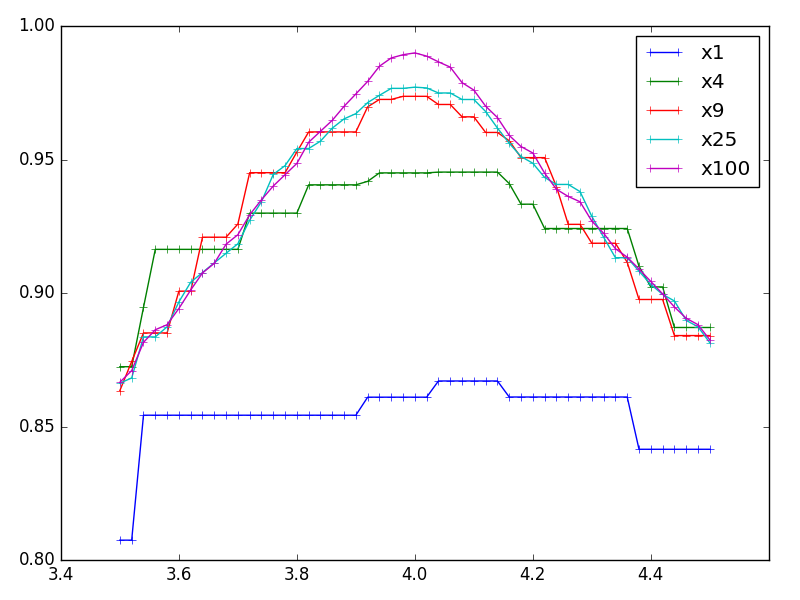
\includegraphics[scale=0.6]{python/ph2/dice/CT-51iter.png}
  \caption{CT: DC of varied radii \& resolutions}
  \label{fig:CT_dc}
\end{figure}

\begin{figure}[!tbp]
  \begin{subfigure}[b]{\textwidth}
    \centering
    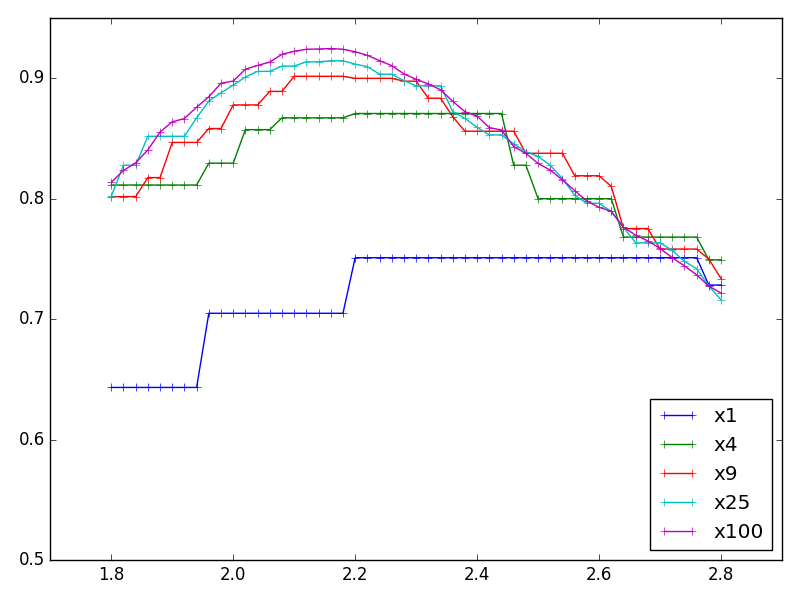
\includegraphics[scale=0.6]{python/ph2/dice/MR-51iter.png}
    \caption{MRI: DC of varied radii \& resolutions}
    \label{fig:MR_dc-opti}
  \end{subfigure}
  \begin{subfigure}[!b]{\textwidth}
    \centering
    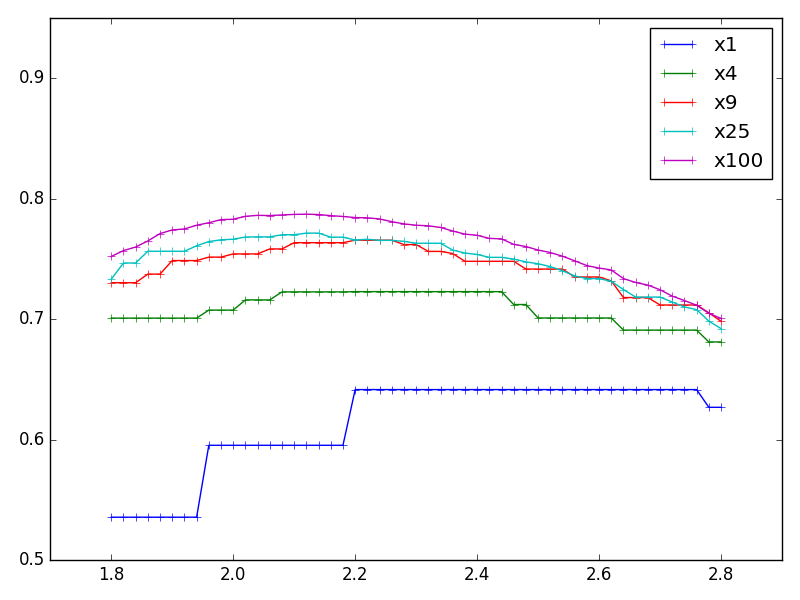
\includegraphics[scale=0.6]{python/ph2/dice/MR_CT-COM_51iter.png}
    \caption{MRI: DC of varied radii \& resolutions (using CT-COM)}
    \label{fig:MR_CT-COM_dc-opti}
  \end{subfigure}
  \caption{}
  \label{fig:MR_dc}
\end{figure}

\clearpage



\subsection{rod \#17}

After deciding which of the possible liquids might be a suitable choice for future use of the phantom, another set of MRI/CT scan was taken.
This second data set shows the rod conatining liquid \#17.
Again it was analysed using the developed script.
Table \ref{tab:spit-out-17} shows the most interesting areas of the rod.

\begin{table}[p]
   \centering
   \rotatebox{90}{
     \begin{minipage}{\textheight}\footnotesize
       \centering
\begin{tabular}{rr|lll|ll|llll}
slice	& dist [$mm$]	& $warp_x$ [$mm$]	& $warp_y$ [$mm$]	& $warpMagnitude$ [$mm$]	& $DC_{CT}$	& $DC^*_{CT}$	& $DC_{MR}$	& $DC^*_{MR}$	& $DC_{MR(CT-COM)}$	& $DC^*_{MR(CT-COM)}$\\ \hline
0     	& -361			& 2.9381	& 0.4266 	& 2.9689			& 0.9486	& 0.9486	& 0.049 	& 0.0251		& 0     			& 0.0054				\\
1     	& -360			& 2.9369	& 0.4257 	& 2.9676			& 0.9517	& 0.9517	& 0.0519	& 0.0266		& 0     			& 0.0054				\\
2     	& -359			& 2.9411	& 0.4186 	& 2.9707			& 0.9537	& 0.9537	& 0.0577	& 0.0296		& 0     			& 0.0069				\\
:     	&     			&       	&        	&       			&       	&       	&       	&       		&       			&       				\\
\hline
:     	&     			&       	&        	&       			&       	&       	&       	&       		&       			&       				\\
351   	& -10 			& -0.205	& -0.034 	& 0.2082			& 0.9869	& 0.9869	& 0.6345	& 0.9123		& 0.6345			& 0.9074				\\
352   	& -9  			& -0.222	& -0.0157	& 0.2228			& 0.984 	& 0.984 	& 0.6352	& 0.9132		& 0.6352			& 0.906 				\\
353   	& -8  			& -1    	& -1     	& -1    			& -1    	& -1    	& 0.6351	& 0.913 		& -1    			& -1    				\\
354   	& -7  			& -1    	& -1     	& -1    			& -1    	& -1    	& 0.6354	& 0.9159		& -1    			& -1    				\\
355   	& -6  			& -1    	& -1     	& -1    			& -1    	& -1    	& 0.6325	& 0.9164		& -1    			& -1    				\\
356   	& -5  			& -1    	& -1     	& -1    			& -1    	& -1    	& 0.6303	& 0.8983		& -1    			& -1    				\\
357   	& -4  			& -1    	& -1     	& -1    			& -1    	& -1    	& 0.6273	& 0.9005		& -1    			& -1    				\\
358   	& -3  			& -1    	& -1     	& -1    			& -1    	& -1    	& 0.6238	& 0.902 		& -1    			& -1    				\\
359   	& -2  			& -1    	& -1     	& -1    			& -1    	& -1    	& 0.6275	& 0.9069		& -1    			& -1    				\\
360   	& -1  			& -1    	& -1     	& -1    			& -1    	& -1    	& 0.6314	& 0.9116		& -1    			& -1    				\\
361   	& 0   			& -1    	& -1     	& -1    			& -1    	& -1    	& 0.6361	& 0.9131		& -1    			& -1    				\\
362   	& 1   			& -1    	& -1     	& -1    			& -1    	& -1    	& 0.6402	& 0.9008		& -1    			& -1    				\\
363   	& 2   			& -1    	& -1     	& -1    			& -1    	& -1    	& 0.6365	& 0.9012		& -1    			& -1    				\\
364   	& 3   			& -1    	& -1     	& -1    			& -1    	& -1    	& 0.6325	& 0.9021		& -1    			& -1    				\\
365   	& 4   			& -1    	& -1     	& -1    			& -1    	& -1    	& 0.6291	& 0.9014		& -1    			& -1    				\\
366   	& 5   			& -1    	& -1     	& -1    			& -1    	& -1    	& 0.6251	& 0.9002		& -1    			& -1    				\\
367   	& 6   			& -1    	& -1     	& -1    			& -1    	& -1    	& 0.6236	& 0.9029		& -1    			& -1    				\\
368   	& 7   			& -1    	& -1     	& -1    			& -1    	& -1    	& 0.6223	& 0.9047		& -1    			& -1    				\\
369   	& 8   			& -1    	& -1     	& -1    			& -1    	& -1    	& 0.6204	& 0.9073		& -1    			& -1    				\\
370   	& 9   			& -1    	& -1     	& -1    			& -1    	& -1    	& 0.6223	& 0.9124		& -1    			& -1    				\\
371   	& 10  			& -1    	& -1     	& -1    			& -1    	& -1    	& 0.626 	& 0.9173		& -1    			& -1    				\\
372   	& 11  			& -1    	& -1     	& -1    			& -1    	& -1    	& 0.6308	& 0.9219		& -1    			& -1    				\\
373   	& 12  			& -1    	& -1     	& -1    			& -1    	& -1    	& 0.6358	& 0.9275		& -1    			& -1    				\\
374   	& 13  			& -0.251	& 0.1248 	& 0.2807			& 0.9872	& 0.9872	& 0.6366	& 0.9314		& 0.6366			& 0.9161				\\
375   	& 14  			& -0.218	& 0.1171 	& 0.2483			& 0.9866	& 0.9866	& 0.6314	& 0.9333		& 0.6314			& 0.9207				\\
:     	&     			&       	&        	&       			&       	&       	&       	&       		&       			&       				\\
\hline
:     	&     			&       	&        	&       			&       	&       	&       	&       		&       			&       				\\
608   	& 247 			& 3.0119	& 0.8035 	& 3.1173			& 0.9847	& 0.9847	& 0.6293	& 0.9206		& 0.2924			& 0.3756				\\
609   	& 248 			& 3.0734	& 0.7794 	& 3.1707			& 0.9829	& 0.9829	& 0.6354	& 0.9326		& 0.2753			& 0.3594				\\
610   	& 249 			& 3.1421	& 0.7525 	& 3.2309			& 0.9829	& 0.9829	& 0.6424	& 0.9423		& 0.2573			& 0.3422				\\
611   	& 250 			& 3.2212	& 0.7379 	& 3.3047			& 0.9878	& 0.9878	& 0.6487	& 0.9392		& 0.2189			& 0.3063				
\end{tabular}
       \caption{rod \#17: script generated data}
       \label{tab:spit-out-17}
     \end{minipage}
   }
 \end{table}

\todo{PIOTR: create colour coded images}

% \begin{figure}[!tbp]
%   \begin{subfigure}[b]{\textwidth}
%     \centering
%     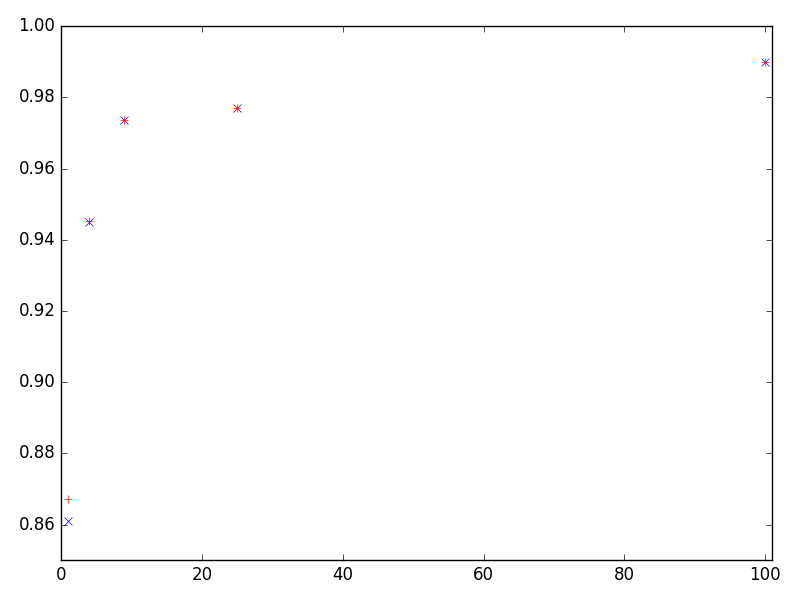
\includegraphics[scale=0.65]{python/ph2/dice/CT_dice-comparison_fast-51iter.png}
%     \caption{CT: x1, x4, x9, x16, x25, x100}
%     \label{fig:MR_dice-comp}
%   \end{subfigure}
%   \begin{subfigure}[b]{\textwidth}
%     \centering
%     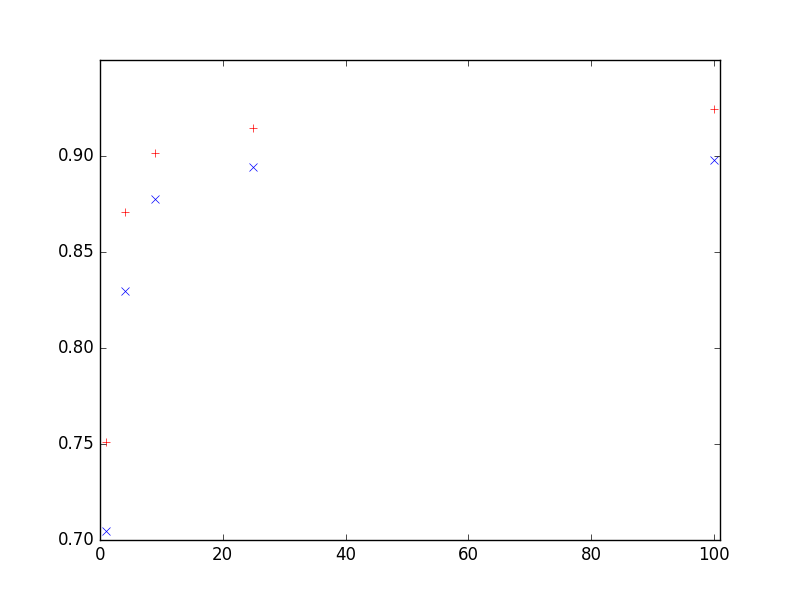
\includegraphics[scale=0.65]{python/ph2/dice/MR_dice-comparison_fast-51iter.png}
%     \caption{MRI: x1, x4, x9, x16, x25, x100}
%     \label{fig:MR_dice_comp}
%   \end{subfigure}
%   \caption{}
%   \label{fig:dice_com}
% \end{figure}

% image of COM shift